\chapter{Ideen und Konzepte}
\label{ch:ideen_konzepte}
In diesem Kapitel werden auf die verschiedenen Ideen und Konzepte genauer eingegangen, welche in der Arbeit verwendet
wurden. Es beinhaltet Ideen zu dem verwendeten Datensatz, den verwendeten Modellen und dem Training der Modelle.

\section{Problemdefinition}
\label{sec:Problemdefinition}
Der Aufbau eines Satzes $ S $ kann linguistisch als Semantik und Syntax beschrieben werden.
\noindent
\myequations{Struktur eines Satzes}
\begin{equation}
	S = S_{semantic} + S_{syntax}
	\label{eq:structure_sentence}
\end{equation}
\noindent
Syntax und Semantik in der natürlichen Sprache zu trennen, ist eine Herausforderung. Da vor allem das Erkennen der
Semantik schwierig ist, denn die selben Wörter in unterschiedlichen Kontexten können zur Syntax oder auch zur Semantik
gehören. Zu beachten ist, dass die Syntax einen Einfluss auf die Semantik haben kann. So zum Beispiel das Pronomen \flqq
nichts\frqq \ und das gross geschriebene Substantiv \flqq Nichts\frqq. So kann der Transfer, welcher \flqq positive\frqq
in \flqq negative\frqq \ Sätze wandelt, die Semantik des Ausgabesatzes beeinflussen. Jedoch möglichst den Bezug zum
Kontext, dem positiven oder negativen Subjekt, zu wahren.
\newline
\newline
Der Input des zu erarbeitenden Prototypen des Zeugnismanagers, ist die Bewertung $ c_{P} $ einer Person $ P $ sowie eine
Eingabesequenz $x$. Diese Bewertung $c_P$ ist dem Kontext eines Satzes gleich zu stellen, und soll beim Transfer nicht
geändert werden. Ausserdem wird jeder Satz einem stylistischen Label $y$ zugeordnet. Aus der Bewertung, Stylelabel und dem
Eingabesatz folgt $ x $ welcher aus $c_P$ und $y$ zusammengesetzt ist, ähnlich wie \ref{eq:structure_sentence}.
\noindent
\myequations{Möglichkeiten der Werte der Stillabels}
\begin{equation}
	\begin{split}
		y_k = holprig &= klexikon \\
		&\text{oder} \\
		y_w = flüssig &= wikipedia
	\end{split}
	\label{eq:style_labels}
\end{equation}
\noindent
Diese Labels sind wie in Formel \ref{eq:style_labels} ersichtlich, in $holprig$ und $flüssig$ unterteilt. Dabei soll
$holprig$ bedeuten, dass der Satz aus dem Zeugnismanager generiert wurde und noch gewisse Verbesserungen vorgenommen
werden müssen bevor dieser in ein Arbeitszeugnis einfliessen kann. $flüssig$ hingegen bedeutet, dass die Sequenz
qualitativ hochwertig ist und nicht mehr weiter bearbeitet werden muss. Diesen definierten Labels wurden, aufgrund der
\fullref{sec:abschliessende_problemdefinition} ein synonymes Label zugeordnet, welches den Datensatz
\ref{sec:verwendeter_datensatz} wiederspiegelt. Aus der Anforderung folgt, dass der angestrebte Zielstil $y_w$ ist.
\newline
\newline
Wie aus der \fullref{sub:aufgabenstellung} zu entnehmen ist, entspricht der Stil der Eingabesatzes $x$ dem Stillabel
$y_k$ und soll in den Zielstil $y_w$ transferiert werden, ohne dass dessen Bewertung $c_P$ verloren geht. Somit entsteht
ein neuer transferierter Satz $\hat{x}$.
\myequations{Aufgabenstellung mathematisch formuliert}
\begin{equation}
	\hat{x} = (x - y_k)  + y_w \quad mit \quad y = y_w
	\label{eq:problemdefinition}
\end{equation}

\section{Abschliessende Problemdefinition}
\label{sec:abschliessende_problemdefinition}
Ein Wissenstext für Kinder aus dem Klexikon, unterscheidet sich im Schreibstil zu einem Text für Erwachsene aus
Wikipeida. Durch das Ersetzen von $ holprig $ und $ flüssig $, durch $ klexikon $ und $ wikipedia $ kann ein ähnliches
Problem, wie in \fullref{sec:Problemdefinition} beschrieben, modelliert werden. Wie unter
\fullref{sub:statistische_analyse_des_datensatz} aufgezeigt, beinhalten die Sätze von Wikipedia, Stillabel $ wikipedia
$, mehr Wörter als die Sätze aus dem Klexikon, mit Stillabel $ klexikon $. Daher kann das Problem abschliessend so
beschreiben werden, dass der Style Transfer aus einem kurzen Satz einen längeren Satz mit gleichem, erweiterten Inhalt
generiert. Ensprechendes gilt für den umgekehrten Fall. So sollte die Länge der generierten Sätze aus einem Stillabel
der Verteilung der Länge aus dem Zielstil folgen.

\section{Verwendeter Datensatz}
\label{sec:verwendeter_datensatz}
Um die mögliche Modelle evaluieren zu können, wird ein Datensatz aufbereitet. Für die Gebiete von Arbeitszeugnisse sind
leider zu wenig Daten vorhanden. Eine naheliegende Möglichkeit ist, die Daten eines Lexikon oder andere, weitverbreitete
und vielfach übersetzte Informationen. Die Texte weisen dabei einen zielgruppengerechten Schreibstil auf.
\newline
\newline
Themengebiete aus welchem entsprechende Texte stammen könnten sein,
\begin{enumerate}
	\setlength\itemsep{0em}
	\item Lexikon / Wikiseite
	\item Bibel
	\item Zeitungen
\end{enumerate}
\noindent
Bei der Recherche für eine geeignete Datenquelle, wurden Zeitungen früh ausgeschlossen. Es finden sich keine
praktikablen und einfach zusammentragbaren Kinderzeitungen online. Weiter wären die Themen der Zeitungsartikel sehr
breit aufgestellt. Auch fokussieren sich Kinderzeitungen nicht auf das gleiche Weltgeschehen wie Zeitungen.
\newline
\newline
Aus dem Themengebiet der Religion, namentlich \flqq die Bibel\frqq, finden sich zahlreiche Quellen. Dabei unterscheidet
sich jedoch der Inhalt teilweise enorm. Hierzu werden in Kinderbibeln oft eine vielzahl an Illustrationen verwendet.
Auch sind sie oft als Erzählbücher gestaltet. So unterscheiden sie sich nicht zwingend im Schreibstil, jedoch mehr in
der Wortwahl. Weiter fanden sich wenige Quellen, bei welchen die Daten in einem handhabaren Format aufbereitet sind.
Eine Extraktion der Texte aus PDFs oder gar gebundenen Bücher hätte einen zu grossen Aufwand mit sich gezogen. Daher
wurde die Verwendung der Bibel als Quelle bis auf weiteres zurückgestellt.
\newline
\newline
An Lexikas gibt es eine Vielzahl von Ausgaben. Sowohl für Erwachsene als auch für Kinder. Die naheliegenste Quelle für
Texte für Fortgeschrittene ist, die Online Enzyklopädie \flqq Wikipedia\frqq. Bei der Recherche liess sich ebenfalls ein
Online Lexikon für Kinder finden, das \flqq Klexikon\frqq. Diese beiden Quellen basieren auf dem Open-Source Framework
\flqq WikiMedia\frqq. Entsprechend kann einfach ein Crawler für diese Seiten erstellt werden. Das Klexikon enthält ca.
2'700 Artikel, in einem für Kinder verständlichen Schreibstil. Für nahezu alle Artikel besteht ein korrespondierender
Artikel in Wikipedia. Nach Rücksprache mit der Betreuungsperson hat man sich für die Verwendung dieser Artikel
entschieden. Die Aufbereitung des Datensatzes wird im Kapitel \fullref{ch:Realisierung} beschrieben.

\section{Momentan verfügbare Forschung}
In einem ersten Teil wurde nach bestehenden Forschungen, im Bereich der Problemstellung, gesucht. Es konnten schnell
viele verschiedene Ansätze gefunden werden, um das Problem lösen zu können. Dabei gab es viele unterschiedlichen
Lösungsansätzen, \gls{NST}, \gls{RNN}, Transformer, Fuzzy Logic und noch viele weitere. Es wurde schnell klar, dass das
Gebiet eingeschränkt werden muss, um die Ressourcen des Projektes optimal auszuschöpfen. Das spannendste Teilgebiet war
der \gls{NST}, auf welches sich diese Forschung hauptsächlich konzentrierte.
\newline
\newline
Bei der Suche nach den vielversprechendsten Ansätzen von \gls{NST}, wurden eine Menge an aktuellen Forschungen gefunden,
da das Gebiet als ehr jung gilt. Die meisten dieser Arbeiten fokussieren sich auf die Übertragung von der Stimmungslage
in eine andere, zum Beispiel von einem positiven in einen negativen Satz. Diese Problemdefinition wird im \gls{NST}
immer wieder verwendet um neue Modelle zu testen. Meistens werden dafür Sätze von Bewertungen (z.B. Tripadvisor oder
IMDB) als Datensatz verwendet. Diese Problemstellung dient in den meisten Fällen nur zur Veranschaulichung der
Einsatzmöglichkeiten der Modelle.
\newline
\newline
Bei der Recherche wurde ein sehr gut gepflegtes und aktuelles GitHub Projekt gefunden, welches sich darauf fokussiert,
die neusten wissenschaftlichen Arbeiten, im Gebiet des Style Transfer, zu verlinken. Ausserdem wird immer versucht Code
zu den entsprechenden Werken zu finden und zu verlinken. Das Repository findet sich auf GitHub unter
\hyperlink{https://github.com/fuzhenxin/Style-Transfer-in-Text}{GitHub Style Transfer in Text}
(\cite{fuzhenxin_style_transfer_in_text}).
\newline
Im Projekt werden die Arbeiten in verschiedene Abschnitte unterteilt, je nach dem, um welches Untergebiet es sich
handelt: Dataset, Supervised (Parallel Data), Unsupervised (Non-parallel Data) und Semi-Supervised. Es wurde sehr
schnell klar, dass die Unterlagen im Bereich Supervised und Semi-Supervised nicht erforscht werden müssen, da es sich
bei unserem Datensatz \ref{sec:verwendeter_datensatz} um nicht parallele Daten handelt.
\newline
Im Bereich des Unsupervised Style Transfer, wurden verschiedene Arbeiten, im Bezug auf die Anwendbarkeit auf unsere
Problemdefinition, untersucht. Dabei wurden vor allem die Unterlagen mit entsprechendem Code untersucht, da die
Umsetzung solcher Arbeiten sehr aufwendig ist. Die meisten dieser Papers beschreiben ein spezielles Modell, welches
einen Style Transfer für bestimmte Probleme vornehmen kann. Diese Modelle sind meistens sehr ähnlich aufgebaut und haben
viele Gemeinsamkeiten. Notizen zu den einzelnen Arbeiten kann im Anhang unter \fullref{app:recherche} gefunden werden.
\newline
\newline
Es wurde schnell bemerkt, dass viele der untersuchten Arbeiten immer wieder die Modelle \textbf{ControlGen} und
\textbf{CrossAlign} brauchen um neue exotische Architekturen zu überprüfen, meistens mit der Frage: \glqq Ist die neue
Architektur besser als die allgegenwärtige?\grqq Daher wurde sehr schnell klar, das in diesem Projekt diese Baseline
Modelle verwendet werden sollen, da es sich bei dem Problem um erste Versuche mit \gls{NST} in deutscher Sprache
handelt. Weitere Architekturen können in einem weiterführenden Projekt untersucht werden, übersteigen jedoch den Rahmen
dieses Projektes.
\newline
\newline
Anschliessend wurden die Unterlagen zum ControlGen (\cite{hu2017controlled}) und CrossAlign (\cite{shen2017style})
Modell durchgearbeitet. Beide Arbeiten der Modelle haben auch eine Implementation in Tensorflow, diese wurden auch genau
untersucht, um die Architekturen besser zu verstehen. Sehr schnell wurde bemerkt, dass die Standardimplementationen der
Modelle eher dürftig sind und es wurde weiter gesucht, nach besseren Implementationen.
\newline
Im Repository wurde dann das Paper (\cite{Li2019DomainAT}) gefunden, welches die beiden Architekturen als Baseline
brauchen um ihre domain adaptiven Modelle damit zu vergleichen. Die Arbeit möchte vor allem zeigen, dass es mit ihren
Modellen möglich ist, durch parallele Daten nicht nur den Stil zu erlernen, sondern auch deren Domäne und ihre
Eigenschaften. Die Idee des Projektes ist sehr interessant, jedoch können diese speziellen Modelle nicht auf unseren
Datenkorpus angewendet werde. Das Projekt bietet aber einen hochwertigen Implementation in Python und Tensorflow zu den
beiden Modellen. Daher wurde entschieden dieses Projekt für die Experimente und das weitere Projekt zu verwenden. Das
Original Repository findet sich auf GitHub unter \hyperlink{https://github.com/cookielee77/DAST}{GitHub DAST}
(\cite{cookielee77_dast}).

\subsection{Modelle}
\label{sub:modelle}
Das Repository (\cite{cookielee77_dast}) welches in diesem Projekt verwendet wurde, beinhaltet zwei Style Transfer
Modelle, \fullref{sub:control_gen} und \fullref{sub:cross_align}. Diese beiden sind im Grundsatz sehr ähnlich und erben
daher beide vom \fullref{sub:base_model}, daher können die Modelle gleich trainiert, getestet und verwendet werden.
Ausserdem sind die Hyperparameter der beiden Architekturen identisch und können somit gegenüber gestellt werden. Um die
beiden Modelle zu evaluieren, befindet sich in dem Projekt ein \fullref{sub:classifier}. Dieser ist dafür zuständig, zu
überprüfen ob die Sätze zu dem korrekten Style transferiert wurden. Mittels dem Classifier kann daher eine
\textit{transfer accuracy} berechnet werden.
\begin{figure}[H]
	\centering
	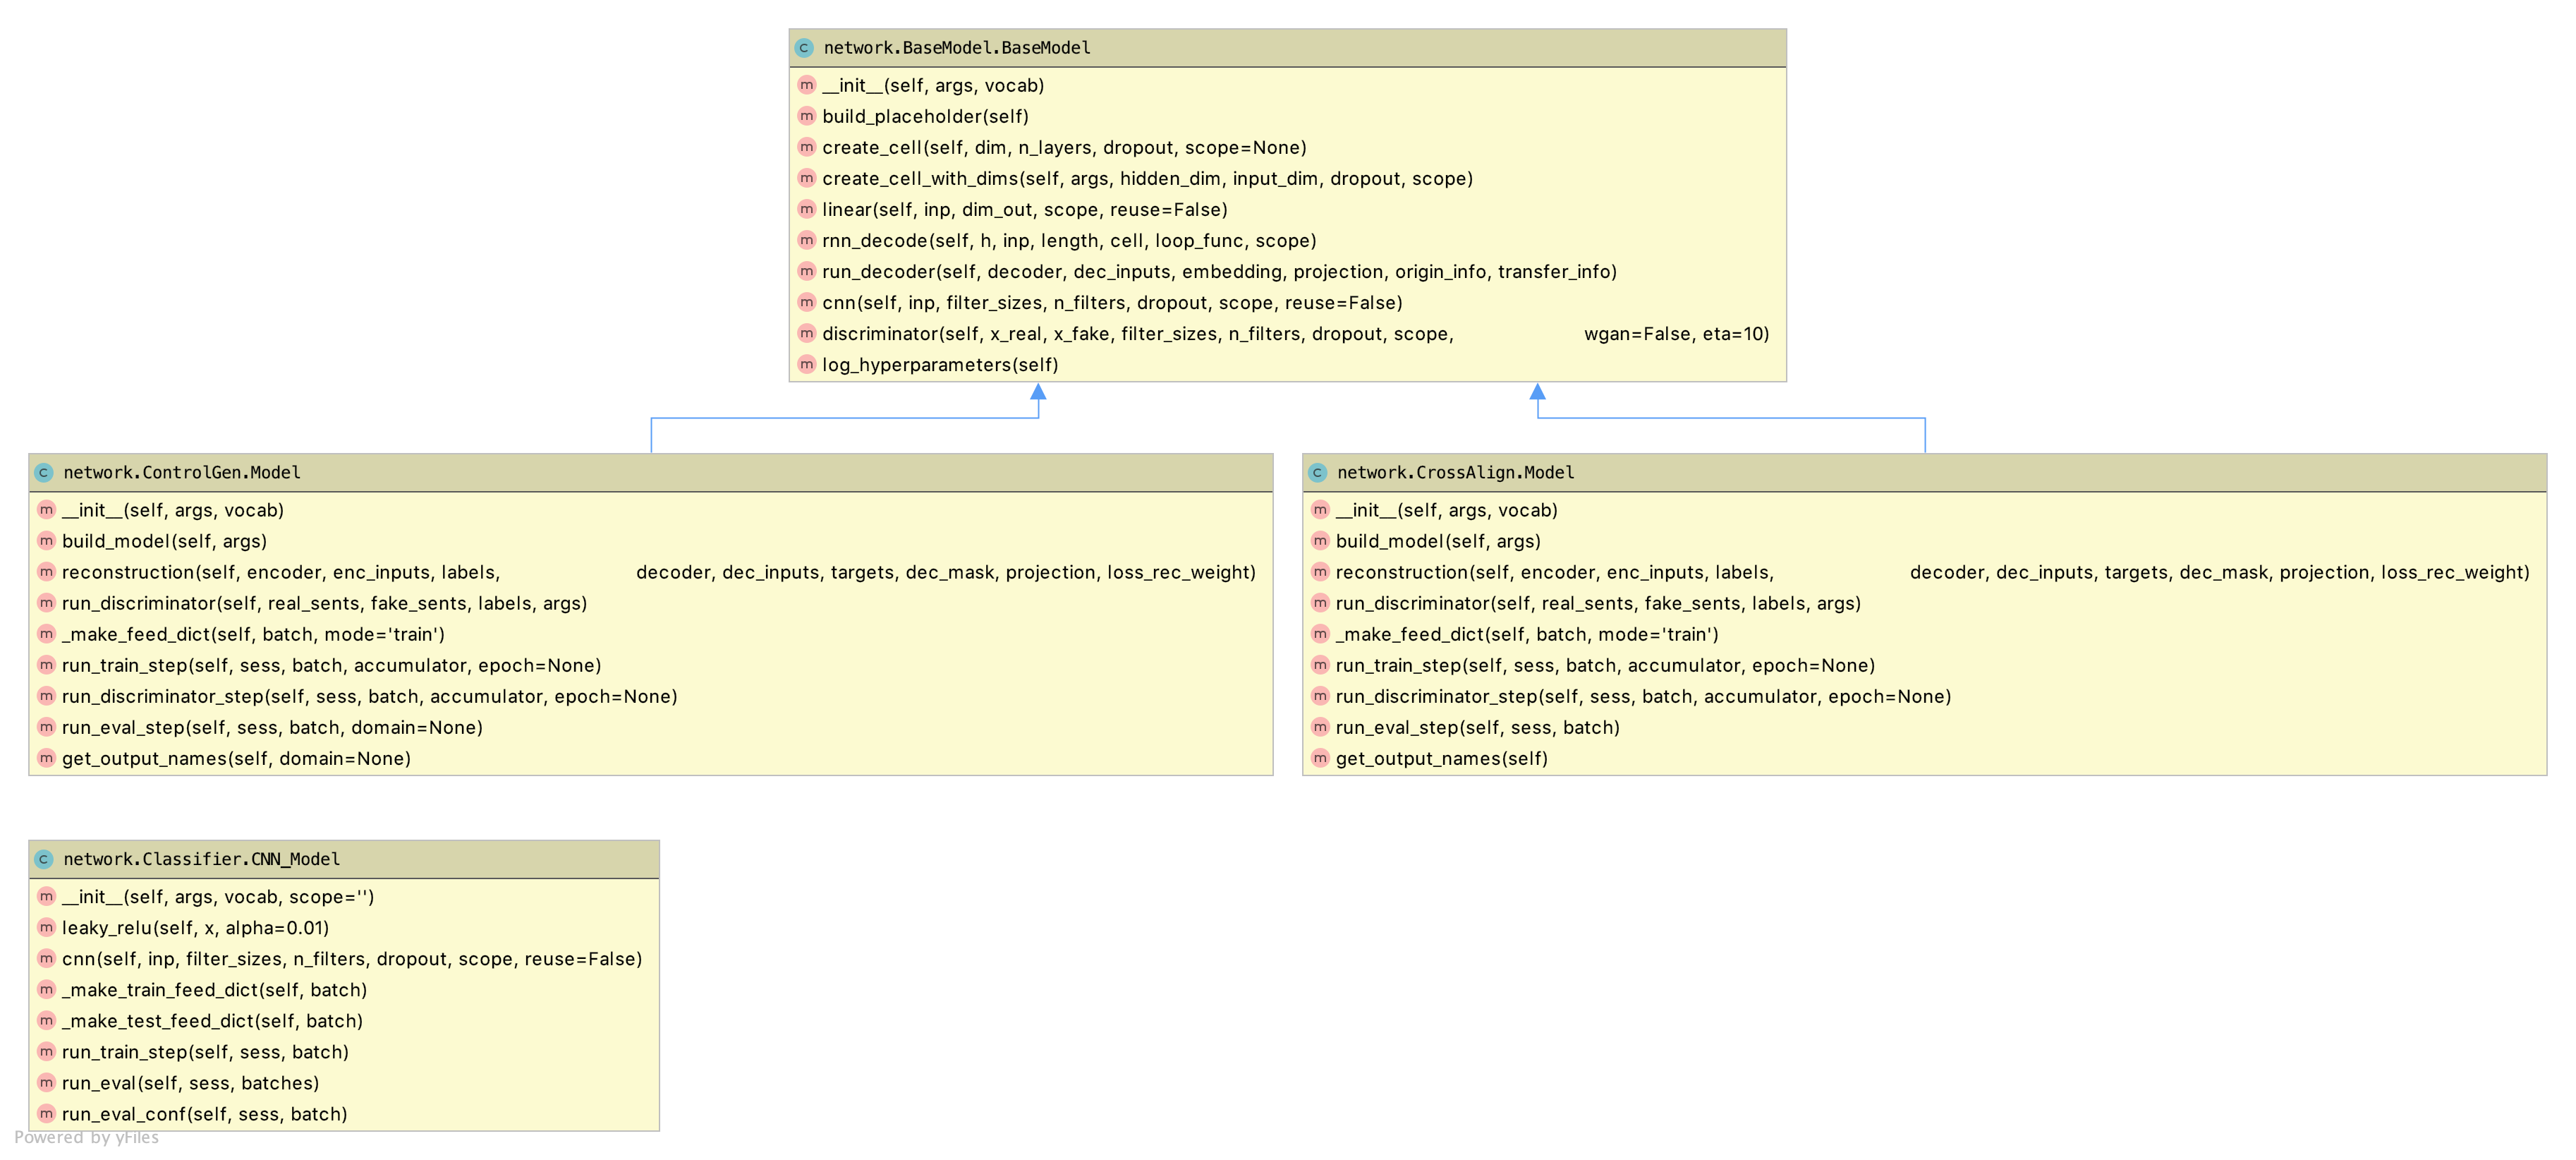
\includegraphics[scale=0.11]{uml_models}
	\caption{Klassendiagramm der Modelle}
	\label{fig:uml_models}
\end{figure}
\noindent
Die Modelle wurden mit dem Datensatz, welcher in \fullref{sec:verwendeter_datensatz} beschrieben wurde, trainiert und
evaluiert. Um diesen Datensatz für das Modell lesbar zu machen, müssen die Sätze in einen Vektor aus IDs transformiert
werden. Jede ID repräsentiert dabei ein Wort, und kann damit eindeutig zugeordnet werden. 
\newline
\newline
Um diese Vektoren zu erstellen, muss als erstes ein Vokabular von den Daten erstellt werden. Dieses beinhaltet alle
Vorkommnisse der einzelnen Wörter im Datenkorpus. Um die Grösse dieses Vokabulars einzuschränken, muss jedes Wort eine
gewisse Anzahl darin vorkommen um aufgenommen zu werden, diese Anzahl an Vorkommnissen ist als
Hyperparameter verfügbar. 
\newline
\newline
Jedem dieser Wörter im Vokabular wird eine eindeutige ID zugeordnet um ein \flqq Wort zu ID\frqq \ und \flqq ID zu
Wort\frqq \ Array zu erstellen. Diese beiden Arrays werden danach genutzt um die einzelnen Sätze in ID Vektoren zu
transformieren und wieder zurück. Wenn nun ein Wort, welches das minimale Vorkommen im Datenkorpus nicht erreicht hat,
transferiert werden möchte, wird diesem Wort ein Platzhalters zugeordnet, wie zum Beispiel \verb|<unk>|. Dadurch kann es
sein, dass bei der Rekonstruktion der Sätze aus den ID Vektoren solche Platzhalter vorkommen, was in
\fullref{sec:eval_output} ersichtlich ist.

\subsection{Classifier}
\label{sub:classifier}
Der Classifier ist ein \gls{CNN}, welches aus mehreren Schichten mit dem gleichen Aufbau bestehen. Zuerst eine
convolution Schicht gefolgt von der Leaky Relu Aktivierungsfunktion \ref{sub:activation-relu} und zum Schluss noch ein
Max-Pooling Layer. Dieser Aufbau wird mehrmals hintereinander geschaltet. Als Verlustfunktion wird eine Softmax Funktion
verwendet, da es sich bei den Daten um gelabelte Daten, welche entweder $0$ oder $1$ sind, handelt. Als Optimizer wird
hier und im ganzem Projekt Adam verwendet. Das Ziel des Classifiers ist es ein \gls{CNN} zu trainieren um zu
unterscheiden ob es sich bei dem vorliegenden Satz um einen Klexikon oder Wikipedia Satz handelt.
\begin{figure}[H]
	\centering
	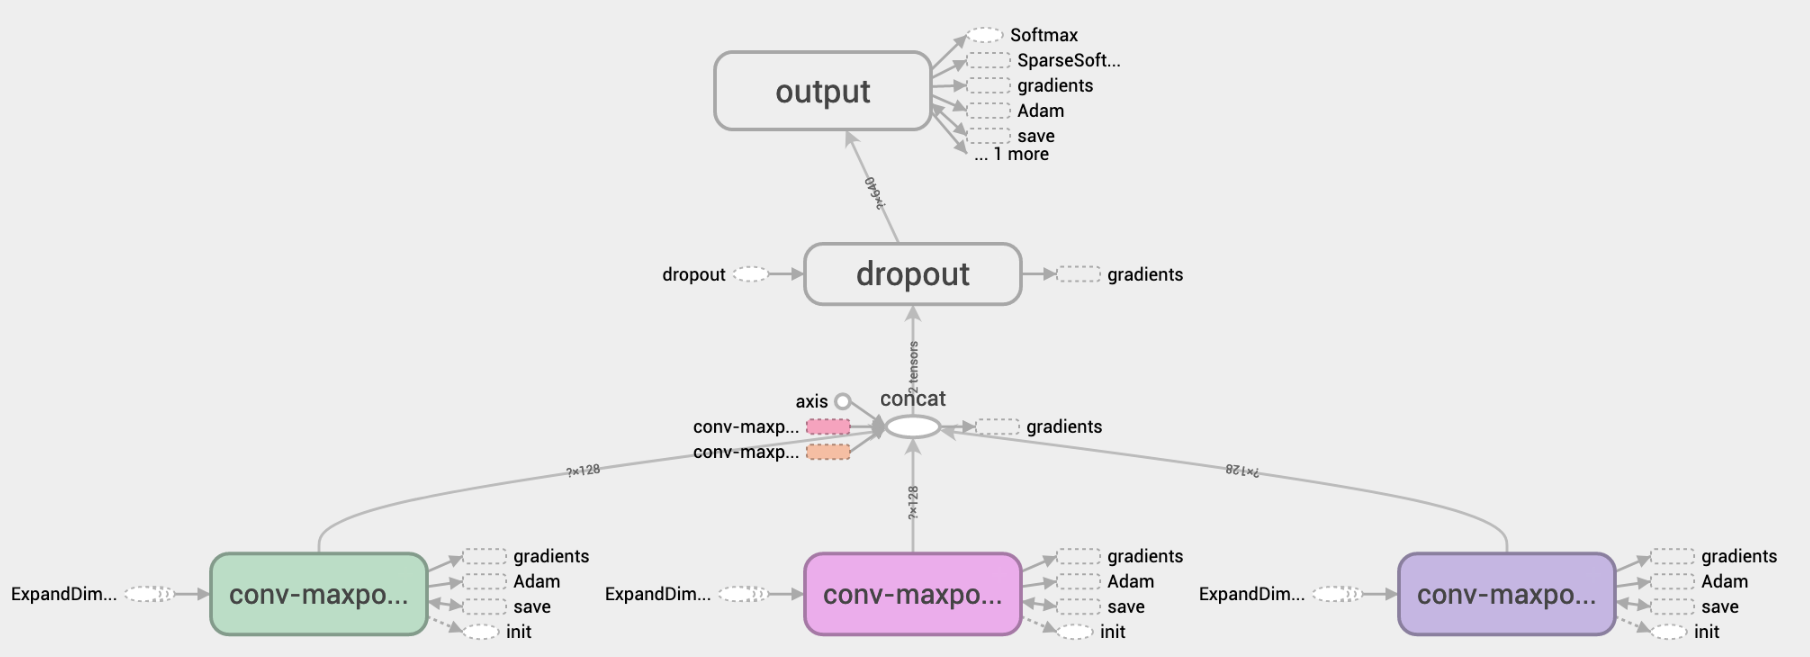
\includegraphics[scale=0.425]{classifier_architecture}
	\caption{Visualisierung der Classifier Architektur}
	\label{fig:classifier_architecture}
\end{figure}
\noindent
Beim Classifier können mit verschiedenen Hyperparameterern unterschiedliche Ergebnisse erzielt werden, je nachdem wie
der Datenkorpus aufgebaut ist und von welcher Grösse dieser ist.
\begin{table}[ht]
	\centering
	\begin{tabular}{| l | l |}
	\hline
	\textbf{Hyperparameter} & \textbf{Interpretation}                                     \\ \hline
	learning rate           & Wie stark die Funktion sich in die Richtung des             \\ 
	                        & Minimums bewegen soll                                       \\ \hline
	dimension embedding     & Dimension des verwendeten Embedding Layers                  \\ \hline
	filter sizes            & Wie gross die einzelnen Filterkernels der Layers sind       \\ \hline
	number of filters       & Anzahl der Filters pro Convolution Schicht                  \\ \hline                     
	\end{tabular}
	\caption{Hyperparameter des Classifiers}
	\label{tab:Hyperparameter_classifier}
\end{table}

\subsection{BaseModel}
\label{sub:base_model}
Das BaseModel wird in beiden Architektur \fullref{sub:control_gen} und \fullref{sub:cross_align} verwendet, um ein
objektorientierter Ansatz zu verfolgen. Dieses Modell ist nicht vollständig und kann nicht ohne weitere Implementationen
trainiert werden, es dient nur der Abstraktion. In diesem Modell werden alle Hyperparameter für die geerbten Modelle zur
Verfügung gestellt, sowie die wichtigsten Variablen definiert, Dropout, Batch Länge, Encoder Inputs, Decoder Inputs und
noch viele weitere. Ausserdem beinhaltet das Base Modell Implementationen zu den wichtigsten Bestandteile der Netwerke.
Wie zum Beispiel die Implementation einer einzelnen \gls{RNN} Zelle, einer linearen Funktion, einem \gls{CNN} und dem
Diskriminator des \gls{GAN}. Durch das Modell ist es möglich, die verwendeten Hyperparameter der Modelle in einem
lesbaren Format zu loggen.

\subsection{ControlGen}
\label{sub:control_gen}
Das ControlGen Paper (\cite{hu2017controlled}) schlägt ein neues generatives Modell vor, welches \gls{VAE} und Ansätze
eines \gls{GAN} kombiniert um die effektiven semantischen Strukturen von Daten zu erlernen. Mit dieser Kombination soll
das Modell im Stande sein Sätze zu interpretieren und diese mit den gewünschten Eigenschaften zu transformieren. Dabei
soll ein besonderes Augenmerk darauf gelegt werden, dass die Erzeugung der Sätze mittels Merkmale kontrolliert werden
kann.
\newline
\newline
Das Modell zielt darauf ab, plausible Sätze zu erzeugen, die auf Repräsentationsvektoren basieren, die aus bestimmten
semantischen Strukturen aufgebaut sind. Für die Kontrolle des Satzstiles, wird das Modell eine Dimension des
Latentcodes, für den $klexikon$ und $wikipedia$ Stil, zugewiesen. Das Erzeugen des entsprechenden Stils, geschieht
aufgrund der Angabe des entsprechenden Latentcodes. Eine solche Dimension, erfasst immer ein markantes Attribut der
Daten, welches von anderen Merkmalen unabhängig ist.
\newline
\newline
Die ControlGen Architektur baut auf der Struktur eines \gls{VAE} auf, welches aus einem traditionellem Auto-Encoder
besteht, wobei der Latentspace regularisiert wird, um kontrolliert Daten zu erzeugen. Der Encoder des Modelles bekommt
als Input eine Textsequenz $x$, diese wird auf den Latentspace $z$ projiziert, welche die einzelnen Latentcodes $c$ als
Dimensionen enthalten. Die Abbildungen des Inputs auf den Latenspace $z$ sind unstrukturierte Vektoren, welche
reduzierte wichtige Merkmale eines Satzes beinhalten, um diesen wiederherzustellen. Um diese Attribute besser abzubilden
und zu kontrollieren, wird der Latentspace $z$ um eine Reihe von strukturierten Variablen $y$, den Latentcodes, ergänzt,
von denen jede auf ein markantes und unabhängiges semantisches Merkmal abzielt, den Labels der Daten. Diese Latentcodes
$y$ werden im Netzwerk manipuliert um Daten im gewünschten Label zu erzeugen. Der Generator soll von dem kombinierten
Vektor $z$ und $y$ abhängig sein, und generiert Daten welche die semantischen Merkmale des strukturierten Codes $y$
erfüllen. Dieser grobe Ablauf des Modelles ist in Abbildung \ref{fig:control_gen_overview} anschaulich dargestellt.
\begin{figure}[H]
	\centering
	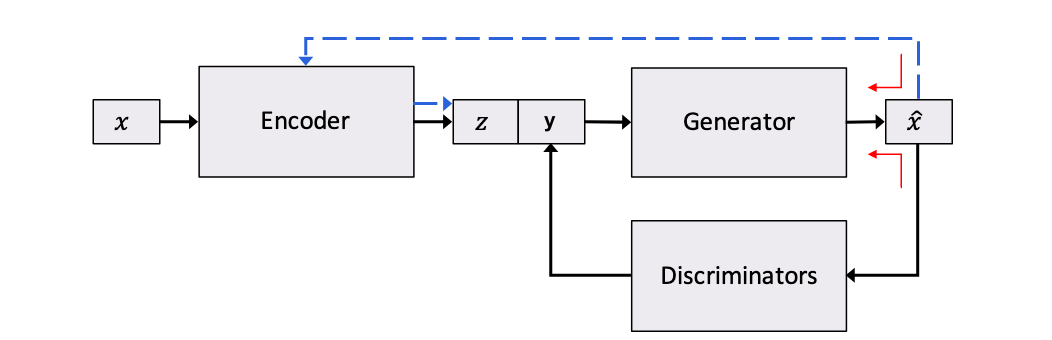
\includegraphics[scale=0.4]{control_gen_overview_edited}
	\caption{Abbildung der Idee von ControlGen}
	\label{fig:control_gen_overview}
\end{figure}
\noindent
Für jedes Merkmal (Label) in $y$ gibt es einen individuellen Diskriminator, um zu messen, wie gut die erzeugten Daten
mit den gewünschten Attributen übereinstimmen. Ausserdem werden diese Diskriminatoren gebraucht um die semantische
Struktur der einzelnen Codes zu entschlüsseln. Dies soll wiederrum den Generator dazu antreiben, bessere Ergebnisse zu
erzeugen, sowie den Latentcode anzupassen.
\newline
\newline
Wenn es einen interpretierbaren Code $y$ gibt, welcher den Output des Generators kontrolliert, muss sichergestellt
werden, dass die verschiedenen Codes nicht voneinander abhängen und sich gegenseitig beeinflussen. Dies ist vor allem
das Problem bei Attributen, welche nicht explizit abgebildet werden möchten. Diese Unabhängigkeit wird erreicht durch
Erzwingen, dass die irrelevanten Attribute vollständig im unstrukturierten Code $z$ abgebildet werden müssen.
\newline
\newline
Durch die Aufteilung des Latentspaces in unstrukturierten Code $z$ und strukturierten Code $y$ kann die Generierung der
Daten vollständig kontrolliert werden. Wenn der Code $y$ gleich bleibt und $z$ zufällig generiert wird, können zum
Beispiel Sequenzen erzeugt werden, welche die gleichen Attribute haben (z.B. $klexikon$, $wikipedia$) jedoch vom Inhalt
komplett verschieden sind. Ausserdem ist es durch diese Aufteilung möglich, den Style Transfer zu kontrollieren. Wenn
ein Satz durch den \gls{VAE} Encoder auf den unstrukturierten Code $z$ abgebildet wird und nur der strukturierte Code
(Label) $y$ abgeändert wird, ist es möglich diese beiden Inputs dem Generator zu übergeben. Dieser generiert daraus ein
Satz, welcher das gleiche Aussagt, jedoch sein Stil (strukturiertes Attribut) geändert wurde.
\newline
\newline
Der Latentcode $(z, y)$ wird aus den Daten erlernt. Der unstrukturierte Code $z$ wird durch ein unsupervised Training
(d.h. die Daten müssen keine Labels enthalten) erlernt durch das konstante Feeback der Diskriminatoren. Wobei der
strukturierte Code $y$ gelabelte Daten (Supervised) braucht um trainiert zu werden, denn $y$ soll die semantischen
Attribute der Sequenzen so optimal wie möglich abbilden.

\subsubsection{Hyperparameter}
\label{sub:crontrol_gen_hyperparameter}
In diesem Abschnitt werden die einzelnen Hyperparameter und deren Interpretation aufgelistet. Diese können verwendet
werden, um die Architektur besser an gewisse Eigenheiten der Problemstellung anzupassen, dies wird Hyperparameter
Optimierung genannt.
\begin{table}[ht]
	\centering
	\begin{tabular}{| l | l |}
	\hline
	\textbf{Hyperparameter} & \textbf{Interpretation}                                     \\ \hline
	max epochs              & Maximale Anzahl an Epochen die das Modell trainiert wird    \\ \hline
	batch size              & Anzahl an Batches in einer Epoche                           \\ \hline
	pretrain epochs         & Wieviele Epochen die Reconstruction und die Diskriminatoren \\
	                        & trainiert werden soll                                       \\ \hline
	learning rate           & Wie stark die Funktion sich in die Richtung des             \\ 
	                        & Minimums bewegen soll                                       \\ \hline
    max length sentences    & Maximale Länge der einzelnen Sätze                          \\ \hline  
	dropout rate            & Wie gross der Dropout des Modelles ist                      \\ \hline
	number of layers        & Wie viele Schichten der Encoder und Decoder haben           \\ \hline
	loss rec weight         & Wie stark der Reconstruction Loss gewichtet wird            \\ \hline
	trim padding            & Ob die generierten und echten Sätze von der selben          \\
	                        & Länge sein sollen                                           \\ \hline
	word embedding          & Welches Word Embedding verwendet werden soll, ob es gelernt \\
	                        & wird als Embedding Layer oder Fasttext verwendet wird       \\ \hline
	dimension embedding     & Dimension des verwendeten Embedding Layers                  \\ \hline
	dimension y             & Dimension des strukturierten Latentcode $y$                 \\ \hline
	dimension z             & Dimension des unstrukturierten Latentspace $z$              \\ \hline
	$\rho$ (rho)            & Wie stark der Generator Loss gewichtet werden soll          \\ \hline        
	$\gamma$ (gamma)        & Wie grosser Anteil der Softmax Funktion im Decoder ist      \\ \hline
	filter sizes            & Wie gross die einzelnen Filterkernels der Layers sind       \\ \hline
	number of filters       & Anzahl der Filters pro Convolution Schicht                  \\ \hline             
	\end{tabular}
	\caption{Hyperparameter des ControlGen Modell}
	\label{tab:hyperparameter_control_gen}
\end{table}

\subsection{CrossAlign}
\label{sub:cross_align}
In der wissenschaftlichen Arbeit (\cite{shen2017style}) in welcher die CrossAlign Architektur vorgestellt wird, ist der
Fokus auf dem Übertragen von Stilen aufgrund von nicht-parallelen Daten. Darin wird das Trennen von Stil und Inhalt als
grösste Herausforderung gesehen, welches mittels dem neu entwickelten Modell gelöst werden soll.
\newline
\newline
Um ein Attribut des Satzes, wie z.B. den Stil, unabhängig vom Inhalt zu kontrollieren, muss es möglich sein den Stil von
anderen Attributen vollständig zu lösen. Das Problem ist jedoch, dass viele verschiedene Attribute miteinander
interagieren, vor allem in Sprachen, wo die Grammatik eine wichtige Rolle spielt.
\newline
\newline
Das Ziel dieses Modells ist es, die Verteilungsäquivalenz von Inhalten zu nutzen, um einen Satz in einem Stil auf einen
stilunabhängigen Inhaltsvektor abzubilden und diesen dann in einen Satz mit dem gleichen Inhalt, aber einem anderen Stil
zu dekodieren. Diese Verteilungsäquivalenz nimmt nur an, dass die Daten in den beiden unabhängigen Domänen die selbe
Verteilung des Inhaltes haben.
\newline
\newline
Das Netzwerk besteht aus einem Encoder, welcher einen Satz und seinen ursprünglichen Stil als Eingabe nimmt und diesen
auf eine stilunabhängige Inhaltsrepräsentation abbildet. Sowie stilabhängige Generatoren, welche die
Inhaltsrepräsentation ohne Stil zu einer Repräsentation mit Stil umwandeln. Für diesen Prozess werden keine typischen
\gls{VAE} verwendet, da es zwingend notwendig ist, die Darstellung der latenten Inhalte reichhaltig und störungsfrei
abzubilden.
\begin{figure}[H]
	\centering
	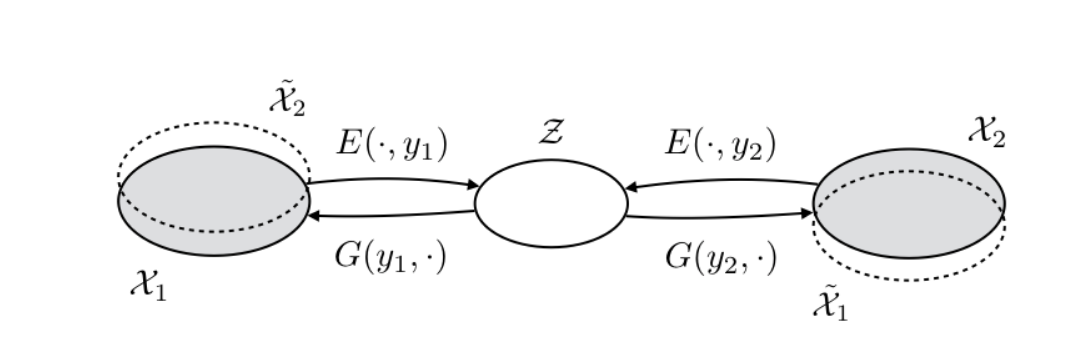
\includegraphics[scale=0.35]{cross_align_overview}
	\caption{Abbildung der Idee von CrossAlign}
	\label{fig:cross_align_overview}
\end{figure}
\noindent
In Abbildung \fullref{fig:cross_align_overview} ist die allgemeine Idee von der CrossAlign Arbeit ersichtlich. $X_1$ und
$X_2$ sind zwei Datensätze mit unterschiedlichen Stilen $y_1$ und $y_2$, z.B. $y_1 = klexikon$ und $y_2 = wikipedia$.
$Z$ ist der gemeinsame Latentspace. Der Encoder $E$ projiziert eine Sequenz auf den gemeinsamen Latenspace $Z$ und
Generator $G$ generiert den Satz zurück wenn dieser mit dem ursprünglichen Stil kombiniert wird. Wenn eine
Inhaltsrepräsentation mit einem anderen Stil dem Generator übergeben wird, transferiert dieser die Sequenz in einen
anderen Stil $\tilde{X_1}$. 
\newline
\newline
Im Datensatz $X$ gibt es verschiedene Sequenzen $X = \{x^{(1)},..., x^{(n)} \}$ welche von der gleichen bedingten Verteilung
$p(x|y,z)$ stammen. Diese Verteilung hängt von der Latent Style Variable $y$ und der Latent Content Variable $z$ ab,
wobei beide Variablen unbekannt sind. Wichtig ist, dass $X$, der aus verschiedenen Stilen generiert
wird, unterschiedlich genug sein sollte, da sonst die Transferaufgabe zwischen den Stilen nicht gut definiert ist. Dies
erscheint zwar trivial, kann aber auch bei vereinfachten Datenverteilungen nicht immer gelten.

\subsubsection{Hyperparameter}
\label{sub:crontrol_gen_hyperparameter}
In diesem Abschnitt werden die einzelnen Hyperparameter und deren Interpretation aufgelistet. Diese können verwendet
werden, um die Architektur besser an gewisse Eigenheiten der Problemstellung anzupassen, dies wird Hyperparameter
Optimierung genannt.
\begin{table}[ht]
	\centering
	\begin{tabular}{| l | l |}
	\hline
	\textbf{Hyperparameter} & \textbf{Interpretation}                                     \\ \hline
	max epochs              & Maximale Anzahl an Epochen die das Modell trainiert wird    \\ \hline
	batch size              & Anzahl an Batch in einer Epoche                             \\ \hline
	learning rate           & Wie stark die Funktion sich in die Richtung des             \\ 
	                        & Minimums bewegen soll                                       \\ \hline
    max length sentences    & Maximale Länge der einzelnen Sätze                          \\ \hline  
	dropout rate            & Wie gross der Dropout des Modelles ist                      \\ \hline
	number of layers        & Wie viele Schichten der Encoder und Decoder haben           \\ \hline
	loss rec weight         & Wie stark der Reconstruction Loss gewichtet wird            \\ \hline
	trim padding            & Ob die generierten und echten Sätze von der selben          \\
	                        & Länge sein sollen                                           \\ \hline
	word embedding          & Welches Word Embedding verwendet werden soll, ob es gelernt \\
	                        & wird als Embedding Layer oder Fasttext verwendet wird       \\ \hline
	dimension embedding     & Dimension des verwendeten Embedding Layers                  \\ \hline
	dimension y             & Dimension des strukturierten Latentcode $y$                 \\ \hline
	dimension z             & Dimension des unstrukturierten Latentspace $z$              \\ \hline
	$\rho$ (rho)            & Wie stark der Generator Loss gewichtet werden soll          \\ \hline        
	$\gamma$ (gamma)        & Wie grosser Anteil der Softmax Funktion im Decoder ist      \\ \hline
	filter sizes            & Wie gross die einzelnen Filterkernels der Layers sind       \\ \hline
	number of filters       & Anzahl der Filters pro Convolution Schicht                  \\ \hline             
	\end{tabular}
	\caption{Hyperparameter des CrossAlign Modell}
	\label{tab:hyperparameter_cross_align}
\end{table}

\section{Training der Modelle}
\label{sec:training_der_modelle}

In diesem Kapitel, \fullref{sec:training_der_modelle}, wird der Aufbau des Trainings der Modelle beschrieben. Es geht
darum die Modelle aus \fullref{sub:modelle} auf den in \fullref{sec:aufbau_datensatz} aufgebauten Datensätzen zu
trainieren. Die Resultate und Weiterführungen der einzelnen Trainings werden in \fullref{sec:resultate} vorgestellt.

\subsection{Verwendete Codebasis}
\label{sub:verwendete_codebasis}

Für das Training der Modelle wurde eine bestehende Codebasis verwendet. Dies aufgrund fehlender Ressourcen, sowie
Erfahrung, eine neue Implementation für die Modelle zu entwickeln. Als Codebasis dient das Github-Repository der
Forschungsgruppe (\cite{Li2019DomainAT}) verwendet. Das Original Repository findet sich auf GitHub unter
https://github.com/cookielee77/DAST (\cite{cookielee77_dast}).
\newline
\newline
Die Codebasis wurde zwecksmässig angepasst. Dabei wurden nicht verwendete Codeteile entfernt. Weiter wurden die Basis
mit für das Projekt nötige Implementation angepasst. Die ursprüngliche Base beinhaltet dabei die Implementation für das
Modell aus \fullref{sub:control_gen} und \fullref{sub:cross_align}. Die Implementationen sind mit Python (\cite{python})
und Tensorflow (\cite{tensorflow}) umgesetzt. 
\newline
\newline
Dabei wurde für die Umsetzung des Wirtschaftsprojekt folgende Erweiterungen für die Codebasis implementiert.

\begin{itemize}
  \setlength\itemsep{0em}
  \item Erweiterung des Projektes mit einem Prototyp um die Modelle manuell zu testen
  \item Erweiterung der Trainings und Evaluations Metriken mit \gls{METEOR} und \gls{WER}
  \item Erweiterung der Funktionalität vom Embedding Layer der einzelnen Modellen, um Fasttext zu verwenden
  \item Kontrolle über die Gewichtung des Reconstruction Loss
  \item Kontrolle über die Anzahl der minimalen Vorkommnisse der Wörter im Vokabular
  \item Umfangreiche Unittests der einzelnen Modelle
  \item Logging der Hyperparameter
  \item Visualisierung der einzelnen Modelle auf dem Tensorboard
\end{itemize}
\noindent

\subsection{Verwendete Trainingsumgebung}
\label{sub:verwendete_trainingsumgebung}
Um ein effizientes Training der Modelle zu ermöglichen, sind entsprechend Rechenressourcen notwending. Privat standen
keine aussreichende Rechener zur verfügung um das Training durchzuführen. Um eine möglichst flexible Gestaltung der
Zeiten für das Training zu ermöglichen, wurde entschieden auf http://vast.ai (nachfolgend vast.ai) zurückzugreifen. Bei
vast.ai können Grafikkarten für Berechnungen angemietet werden. Diese werden über ein Docker Container bereitgestellt.
Der benötigte Code, sowie der Datensatz, wurden in den Container eingespielt. Anschliessend konnte für die Mietdauer die
Grafikkarte verwendet werden. Dabei wurden Grafikkarten vom Typ Nvidia GeForce (\cite{wikipedia_2019_geforce}) verwendet, hauptsächlich die Modelle
Titan X und 1080Ti.

\subsection{Trainingsplanung}
\label{sub:ablauf_und_resultate}
Damit die Trainings der Modelle einem geregeltem Ablauf folgen, wird eine Trainingsplanung durchgeführt. Wie in
\ref{sec:resultate} eingesehen werden kann, geht es darum, die Hyperparameter der beiden Modelle anzupassen. Damit
sollen die Modelle den \gls{NST} auf den beiden Datensatz möglichst genau durchführen. Weiter werden zu Beginn, wie in
\ref{sub:standard_hyperparameter} beschrieben, die Modelle auf beiden Datensätzen, \flqq Ausgeglichen\frqq \ und \flqq Gekürzt\frqq,
trainiert. Auch sollen zuerst die standard Hyperparameter der Autoren der beiden Ansätze verwendet werden. So können die
Modelle ein erstes Mal auf ihre Leistung geprüft werden. Anschliessend können aufgrund der Ergebnisse der ersten
Trainings die Hyperparameter angepasst werden. Um die Resultate gegeneinader vergleichbar zu halten, werden alle
Trainings mit $ 200 $ \gls{Epoche} trainiert.
